% Imporditud: tools/import_eksperimendid.py
% Allikas: Eesti füüsikaolümpiaadi eksperimendi ülesannete
%   kogu (Rael Kalda, 2023), ülesanne Ü2, lahendus L2.
\setAuthor{EFO žürii}
\setRound{piirkonnavoor}
\setYear{1997}
\setNumber{P E1}
\setDifficulty{1}
\setTopic{kinemaatika}
\setVahendid{koormis, nöör, statiiv, mõõtejoonlaud, stoppkell}
\setPunktid{8}
\setAllikas{Eksperimendi kogu Ü2, lahendus lk 34}
\setLahendusseis{toores}

\prob{Koormise keskmine kiirus}
Koormis riputati nööri otsa ja viidi asendisse, kus niit on horisontaalne. Pärast lahti laskmist hakkas koormis võnkuma. Määrata koormise liikumise keskmine kiirus. Analüüsida tulemust mõõtetäpsuse seisukohast.
\begin{center}
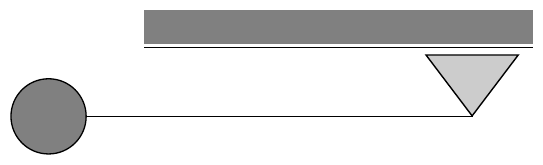
\includegraphics[width=0.36\linewidth]{1997-v2g-pe1-yl.png}
\end{center}

\hint

\solu
Mõõtmised: Mõõdetkse nööri pikkus R (1 p). Mõõdetakse n perioodi kestus t (1 p).

Arvutused: t

Ühe perioodi kestus T = n (1 p). Teepikkus ühe perioodi jooksul L = 2$\pi$R (1 p). L

Keskmise kiiruse valem v = (1 p). T

Vea analüüs: Nööri pikkust mõõtsime täpsusega 0,5 mm (1 p). Perioodi kestuse mõõtmise täpsus sõltub sellest, kui suur oli n (1 p). Ta peab olema piisavalt suur, et keskmistamisel väheneks perioodi mõõtmise viga ja ei tohi olla nii suur, et jõuaks oluliselt väheneda võnkumiste amplituud. Optimaalne n väärtus sõltub ka valitud nööri pikkusest. (1 p)
\probend
